\documentclass{beamer}

\usetheme{Boadilla}

\usepackage[utf8]{inputenc}
\usepackage[T1]{fontenc}
\usepackage[english]{babel}
\usepackage{amsmath, amssymb, mathtools}
\usepackage{graphicx}
\usepackage{lmodern}
\usepackage{tikz}
\usetikzlibrary{arrows.meta, positioning}

\definecolor{LMUGreen}{RGB}{0,136,58}
\definecolor{Black}{RGB}{35,35,35}
\definecolor{White}{RGB}{255,255,255}
\definecolor{Lightgrey}{RGB}{230,230,231}
\definecolor{Middlegrey}{RGB}{192,193,195}

\setbeamercolor{item projected}{bg=LMUGreen,fg=White}
\setbeamercolor{section in toc}{fg=Black,bg=White}
\setbeamercolor{alerted text}{fg=LMUGreen}
\setbeamercolor*{palette primary}{fg=LMUGreen,bg=Lightgrey}
\setbeamercolor*{palette secondary}{fg=LMUGreen,bg=Lightgrey}
\setbeamercolor*{palette tertiary}{bg=LMUGreen,fg=White}
\setbeamercolor*{palette quaternary}{fg=LMUGreen,bg=Black}
\setbeamercolor{titlelike}{parent=palette primary,fg=LMUGreen}
\setbeamercolor{frametitle}{bg=Lightgrey, fg=LMUGreen}
\setbeamercolor{frametitle right}{bg=Middlegrey}

\beamertemplatenavigationsymbolsempty

\setbeamertemplate{footline}
{
  \leavevmode%
  \hbox{%
  \begin{beamercolorbox}[wd=.9\paperwidth,ht=2.25ex,dp=1ex,center]{author in head/foot}%
    \insertsectionnavigationhorizontal{.7\paperwidth}{}{}%
  \end{beamercolorbox}%
  \begin{beamercolorbox}[wd=.1\paperwidth,ht=2.25ex,dp=1ex,right]{date in head/foot}%
    \insertframenumber{} / \inserttotalframenumber\hspace*{2ex}
  \end{beamercolorbox}}%
  \vskip0pt%
}

\title{\texorpdfstring{$D(SP)^2$}{DSP2} -- Status do Projeto}
\subtitle{Biblioteca DSP, conversão áudio-MIDI e orquestra de motores de passo}
\author{Caio Davi de Andrade Monteiro, Rodrigo de Souza Oliveira, Luis Rafael Sena}
\institute{Engenharia Eletrônica e de Computação}
\date{\today}

\newcommand{\imageorplaceholder}[3]{%
    \IfFileExists{#1}{%
        \includegraphics[width=#2\textwidth,height=#3\textheight,keepaspectratio]{#1}%
    }{%
        \fbox{\parbox[c][#3\textheight][c]{#2\textwidth}{\centering
        Arquivo esperado:\\\texttt{#1}}}%
    }%
}

\begin{document}

\begin{frame}
    \titlepage
\end{frame}

\section{Biblioteca}

\begin{frame}{Código geral da biblioteca}
    O núcleo do projeto já está estruturado como uma biblioteca DSP híbrida:
    core em C++ para desempenho e bindings em Python para orquestração.

    \vspace{0.25cm}

    \begin{columns}[T,onlytextwidth]
        \begin{column}{0.48\textwidth}
            \begin{block}{Base implementada}
                \begin{itemize}
                    \item grafo dataflow com engine C++;
                    \item roteamento por buffers;
                    \item bindings Python via pybind11;
                    \item build separado para simulação e embarcado.
                \end{itemize}
            \end{block}
        \end{column}
        \begin{column}{0.48\textwidth}
            \begin{block}{Nós e ferramentas}
                \begin{itemize}
                    \item osciladores, filtros e matemática básica;
                    \item FFT, espectro, picos e pitch;
                    \item leitura WAV e exportação MIDI;
                    \item relatórios, gráficos e logger.
                \end{itemize}
            \end{block}
        \end{column}
    \end{columns}

    \vspace{0.15cm}

    \begin{alertblock}{Validação}
        O repositório tem 10 arquivos de teste: 5 C++/CTest e 5 Python/unittest,
        somando 81 cenários nomeados.
    \end{alertblock}
\end{frame}

\section{Hardware}

\begin{frame}{Orquestra de passo e hardware}
    \begin{columns}[T,onlytextwidth]
        \begin{column}{0.48\textwidth}
            \begin{itemize}
                \item circuito já projetado e simulado;
                \item componentes principais já foram comprados;
                \item ainda não houve teste físico do hardware;
                \item com a peça final, partimos para montagem e testes.
            \end{itemize}

            \vspace{0.2cm}

            \begin{block}{Ponto importante}
                Hardware e software avançam em paralelo: enquanto a placa pendente
                não chega, seguimos validando a biblioteca e o MIDI.
            \end{block}
        \end{column}
        \begin{column}{0.48\textwidth}
            \centering
            \imageorplaceholder{circuito_simulado.png}{0.98}{0.56}
        \end{column}
    \end{columns}
\end{frame}

\begin{frame}{Componentes da orquestra}
    \begin{columns}[T,onlytextwidth]
        \begin{column}{0.52\textwidth}
            \begin{block}{Comprados}
                \begin{itemize}
                    \item cabo de áudio MIDI USB;
                    \item 6x driver de motor de passo A4988;
                    \item 6x motor de passo NEMA 17 17HS4401;
                    \item placa Nano V3 com pinos soldados.
                \end{itemize}
            \end{block}
        \end{column}
        \begin{column}{0.42\textwidth}
            \begin{alertblock}{Pendente}
                \begin{itemize}
                    \item placa adaptador mini shield para Arduino.
                \end{itemize}
            \end{alertblock}

            \vspace{0.2cm}

            \begin{block}{Estado atual}
                A montagem física começa assim que essa placa chegar.
            \end{block}
        \end{column}
    \end{columns}
\end{frame}

\section{MVP}

\begin{frame}{MVP: música para MIDI}
    O MVP transforma uma música em um arquivo MIDI de um canal, que representa
    um motor lógico no fluxo de software.

    \vspace{0.35cm}

    \begin{center}
        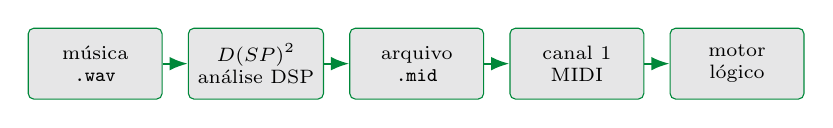
\begin{tikzpicture}[
            node distance=0.32cm,
            flowbox/.style={
                draw=LMUGreen,
                fill=Lightgrey,
                rounded corners=2pt,
                align=center,
                minimum width=1.7cm,
                minimum height=0.9cm,
                font=\scriptsize
            },
            arrow/.style={-Latex, thick, draw=LMUGreen}
        ]
            \node[flowbox] (wav) {música\\\texttt{.wav}};
            \node[flowbox, right=of wav] (lib) {$D(SP)^2$\\análise DSP};
            \node[flowbox, right=of lib] (midi) {arquivo\\\texttt{.mid}};
            \node[flowbox, right=of midi] (ctrl) {canal 1\\MIDI};
            \node[flowbox, right=of ctrl] (motors) {motor\\lógico};

            \draw[arrow] (wav) -- (lib);
            \draw[arrow] (lib) -- (midi);
            \draw[arrow] (midi) -- (ctrl);
            \draw[arrow] (ctrl) -- (motors);
        \end{tikzpicture}
    \end{center}

    \vspace{0.15cm}

    \begin{itemize}
        \item \texttt{peaks}: detecta picos espectrais por bloco.
        \item \texttt{melody}: estima a fundamental e gera uma linha melódica.
        \item saída atual: um canal MIDI, preparado para a primeira validação física.
    \end{itemize}

    \vspace{0.15cm}

    Já temos exemplos \texttt{.mid} gerados no projeto, incluindo testes com
    \textit{Twinkle Twinkle Little Star} e Bach.
\end{frame}

\begin{frame}{Evidência: MIDI gerado}
    \begin{columns}[T,onlytextwidth]
        \begin{column}{0.42\textwidth}
            \begin{block}{O que já funciona}
                \begin{itemize}
                    \item entrada de áudio WAV mono;
                    \item análise espectral e detecção de notas;
                    \item escrita de MIDI em um canal;
                    \item API Python e linha de comando.
                \end{itemize}
            \end{block}
        \end{column}
        \begin{column}{0.54\textwidth}
            \centering
            \imageorplaceholder{midi_musica.png}{0.98}{0.62}
        \end{column}
    \end{columns}

    \vspace{0.2cm}

    \begin{alertblock}{Resultado esperado}
        O arquivo MIDI é a interface entre a biblioteca e a futura montagem:
        primeiro validamos um canal/motor; depois expandimos para vários canais.
    \end{alertblock}
\end{frame}

\section{Integração}

\begin{frame}{Código Arduino}
    \begin{columns}[T,onlytextwidth]
        \begin{column}{0.50\textwidth}
            \begin{itemize}
                \item o código Arduino já está pronto;
                \item ele recebe eventos MIDI;
                \item cada nota é convertida em período de pulso;
                \item o código já prevê o mapeamento por canal/motor.
            \end{itemize}
        \end{column}
        \begin{column}{0.46\textwidth}
            \begin{alertblock}{Estado correto}
                Ainda não testamos o hardware. O Arduino está pronto para teste,
                mas a validação real depende da montagem do circuito.
            \end{alertblock}
        \end{column}
    \end{columns}

    \vspace{0.2cm}

    \begin{block}{Estratégia de validação}
        Primeiro testar um canal MIDI com um motor físico. Depois, ajustar
        temporização e expandir para múltiplos motores sincronizados.
    \end{block}
\end{frame}

\begin{frame}{Integração planejada}
    \begin{columns}[T,onlytextwidth]
        \begin{column}{0.52\textwidth}
            \begin{block}{MVP atual}
                \begin{itemize}
                    \item software gera \texttt{.mid} de um canal;
                    \item esse canal representa um motor lógico;
                    \item ainda não houve teste com motor físico.
                \end{itemize}
            \end{block}
        \end{column}
        \begin{column}{0.42\textwidth}
            \begin{block}{Próxima expansão}
                \begin{itemize}
                    \item canal MIDI 1 $\rightarrow$ motor 1;
                    \item canal MIDI 2 $\rightarrow$ motor 2;
                    \item \dots
                    \item canal MIDI 6 $\rightarrow$ motor 6.
                \end{itemize}
            \end{block}
        \end{column}
    \end{columns}

    \vspace{0.2cm}

    O objetivo depois da validação inicial é sincronizar vários canais para tocar
    acordes com uma voz por motor.
\end{frame}

\section{Próximos passos}

\begin{frame}{Próximos passos}
    \begin{columns}[T,onlytextwidth]
        \begin{column}{0.32\textwidth}
            \begin{block}{Software}
                \begin{itemize}
                    \item refinar estabilidade das notas;
                    \item melhorar detecção melódica;
                    \item preparar MIDI multicanal.
                \end{itemize}
            \end{block}
        \end{column}
        \begin{column}{0.32\textwidth}
            \begin{block}{Hardware}
                \begin{itemize}
                    \item receber o mini shield;
                    \item montar o circuito;
                    \item validar acionamento real.
                \end{itemize}
            \end{block}
        \end{column}
        \begin{column}{0.32\textwidth}
            \begin{block}{Integração}
                \begin{itemize}
                    \item testar primeiro um canal;
                    \item ajustar temporização;
                    \item evoluir para acordes.
                \end{itemize}
            \end{block}
        \end{column}
    \end{columns}

    \vspace{0.45cm}

    \begin{alertblock}{Resumo}
        A parte de software não precisa esperar o hardware terminar: quando o
        mini shield chegar, já teremos a cadeia áudio-MIDI e o Arduino prontos
        para os primeiros testes e ajustes na montagem real.
    \end{alertblock}
\end{frame}

\end{document}
